\subsection{Attività sperimentale: difetto di scia e volume di controllo.}

L'esercizio svolto in precedenza risulta propedeutico per l'analisi dei dati ottenuti tramite alcune attività sperimentali, per ottenere delle risultanti di forze e momenti da misure del campo di velocità (e pressione, a volte) tramite i bilanci integrali.
Le attività svolte nel mondo reale sono affette da imprecisioni e incertezze. La quantificazione (o almeno la stima) dell'incertezza del risultato di un'attività sperimentale è parte integrante del risultato stesso. 
I valori $x_i, \ i=1:N$ di grandezze misurate possono essere combinati per calcolare delle grandezze derivate $f(x_i)$. I \textit{datasheet} che accompagnano uno strumento raccolgono anche le informazioni sulla sua incertezza di misura, spesso in forma di intervallo di confidenza o di scarto quadratico medio. L'incertezza sulle misure sperimentali $x_i$ si propaga sul valore della funzione $f(x_i)$. Nell'ipotesi che le incertezze di misura sulle variabili $d_i$ siano tra di loro indipendenti e non correlate, è possibile utilizzare la \textbf{formula RSS} (\textbf{root-sum-squares}) per la propagazione dell'incertezza. Se la misura $x_i$ ha incertezza $\sigma_{x_i}$, una stima dell'incertezza su $f$ vale
\begin{equation}
  \sigma_f^2 = \sum_{i=1}^{N} \left( \dfrac{\partial f}{\partial x_i} \right)^2 \sigma_{x_i}^2 \ .
\end{equation}
%
L'incertezza $\sigma^2_f$ sulla quantità $f$, obiettivo dell'attività sperimentale, è un indicatore della bontà del metodo sperimentale utilizzato ed del sistema di miusra disponibile per tale attività. In generale, l'incertezza sulla grandezza desiderata deve essere ``molto minore'' della grandezza stessa: in caso contrario, l'apparato sperimentale risulterebbe indeguato all'esperimento.
Essendo parte integrante del risultato, è buona regola indicare l'incertezza sui risultati delle attività sperimentali, ad esempio fornendone il valore numerico, il valore relativo alla misura o gli intervalli di confidenza sui grafici.

% \paragraph{Difetto di scia e resistenza del profilo.}
% \'E possibile stimare la resistenza di un profilo a partire dalla misura del difetto di scia.
%  La misura di velocità in scia viene effettuata (con una sonda di Pitot o altro \dots)
%  in punti discreti, più radi lontano dalla scia del profilo,
%  fiù fitti in corrispondenza della scia dove i gradienti sono maggiori.
% L'integrale nella formula (\ref{eqn:difetto_scia}) viene approssimato con un metodo numerico,
%  come ad esempio la formula del punto medio, quella del trapezio, \dots
% Utilizzando qui per semplicità la formula del punto medio, è possibile scrivere
% \begin{equation}
%  F_x = \int_{0}^{H} \rho u(y) (U_\infty - u(y)) dy
%     \approx \sum_{k=1}^{N} \rho \left[ u_k (U_\infty - u_k) \right] \Delta s_k
% \end{equation}
% Le misure ottenute dalla sonda sono affette da incertezza $\sigma_{u_i}$; la derivata $\partial F_x / \partial u_i$ è
% \begin{equation}
%  \dfrac{\partial F_x}{\partial u_m}  = \rho \left( U_\infty - 2 u_m \right) \Delta s_m
% \end{equation}
% La stima dell'incertezza sulla resistenza è quindi
% \begin{equation}
%  \sigma_{F_x}^2 = \sum_{i=1}^{N} \left[ \rho \left( U_\infty - 2 u_i \right) \Delta s_i \right]^2 \sigma_{u_i}^2
% \end{equation}
% 

\paragraph{Risultante delle forze: bilancio di quantità di moto di un volume di controllo .}
Esistono metodi sperimentali, come ad esempio la \textbf{PIV} (Particle Image Velocimetry o, in italiano, velocimetria a immagini di particelle), che permettono di ottenere il campo di velocità in un determinato istante all'interno di un dominio di misura, un piano bidimensionale o un volume tridimensionale.
Il bilancio di quantità di moto del volume di controllo contenente un corpo solido permette poi di calcolare la risultante delle forze scambiate tra corpo e fluido.

\noindent
 Per semplicità, viene considerato un campo di moto bidimensionale, $\bm{u}(x,y)=u(x,y)\bm{\hat{x}}+v(x,y)\bm{\hat{y}}$. Ad esempio, il campo di moto attorno alla mezzeria di un'ala allungata senza freccia investita da una corrente con un angolo di incidenza ridotto è in buona approssimazione bidimensionale.
 In questo caso, misure PIV (PIV-2D-2C) forniscono le due componenti (2C) del campo di velocità nel piano (2D) di misura. Tramite il bilancio della quantità di moto del dominio bidimensionale, è possibile ottenere una stima della risultante delle forze (per unità di apertura) che esercita il fluido sul profilo di ala tagliato dal piano di misura.
Considerando gli effetti viscosi trascurabili, al di fuori di regioni di dimensione ridotta nell'ambito di applicazioni aeronautiche (alto numero di Reynolds, strato limite e scie sottili), il bilancio integrale della quantità di moto del fluido nel volume di misura fornisce, in un caso stazionario, la risultante delle forze ${\bm{R}}$ agenti sul corpo, 
\begin{equation}
 \bm{R} = -\oint_S \rho \bm{u} \bm{u} \cdot \bm{\hat{n}} - \oint_S p \bm{\hat{n}} \ ,
\end{equation}
avendo trascurato il contributo delle forze di volume.
%
Nell'ipotesi, più che sensata per molte applicazioni aeronautiche, che sia valido il teorema di Bernoulli sulla frontiera $S$ del volume di controllo, la pressione viene espressa in funzione della velocità locale e dello stato della corrente asintotica,
\begin{equation}
 p = p_\infty + \rho \dfrac{|\bm{U_\infty}|^2}{2} - \rho \dfrac{|\bm{u}|^2}{2} \ .
\end{equation}
Inserendo questa espressione della pressione nell'espressione della risultante delle forze ed eliminando gli integrali (nulli) su una superficie chiusa delle quantità costanti moltiplicate per la normale alla superficie, come ad esempio $\oint_S p_\infty \bm{\hat{n}}$, si può esprimere la risultante $\bm{R}$ della forza aerodinamica agente sul corpo in funzione della sola velocità del fluido sulla frontiera $S$,
\begin{equation}
 \bm{R} = -\oint_S \rho \bm{u} \bm{u} \cdot \bm{\hat{n}} + \oint_S \rho \dfrac{|\bm{u}|^2}{2} \bm{\hat{n}} \ .
\end{equation}
Sotto queste ipotesi, la forza aerodinamica agente sul corpo, in questo esempio l'obiettivo della misura, è stata scritta unicamente come funzione del campo di velocità sulla superficie $S$, fornito come ``risultato diretto'' dell'attività seprimentale. Per semplicità, la densità del fluido viene considerata costante e nota senza incertezza: nel caso che anche il campo di densità fosse affetto da incertezza, la formula RSS permette di aggiungere abbastanza facilmente il suo effetto a quello dovuto all'incertezza sulla misura del campo di velocità.
\newline
% TODO: è possible applicare diversi metodi per ricavare un'approssimazione della risultante e della sua incertezza, partendo da dati discreti...
\paragraph{Risultante delle forze: discretizzazione.}
Per la sua natura, la PIV fornisce dei risultati discreti (non continui): di solito, il campo di velocità viene misurato sui nodi di una griglia cartesiana. Per il calcolo della risultante $\bm{R}$ sono necessari solamente gli $N_n$ nodi esterni $\bm{x_i}, \ i=1:N_n$, posti sul contorno della griglia.
% TODO ...
\newline
Il campo di velocità viene approssimato (linearmente, per semplicità) utilizzando un approccio simile a quello impiegato nella modellazione numerica a elementi finiti. Viene introdotto un insieme completo di funzioni di base $\phi_i(\bm{x}), \ i=1:N_{n}$, lineari a tratti sul contorno $S$, grazie alle quali è possibile scrivere l'approssimazione $\bm{u}^h$ del campo di velocità
\begin{equation}\label{exp:u:fem-exp}
 \bm{u}(\bm{x}) \approx \bm{u}^h(\bm{x}) = \displaystyle\sum_{i=1}^{N_n} \phi_i(\bm{x}) \bm{U_i} \ . 
\end{equation}
Utilizzando funzioni di base lagrangiane, per le quali il valore della funzione $i$-esima $\phi_i(\bm{x})$ è uguale a uno sul nodo $i$-esimo $\bm{x}_i$ e zero sugli altri nodi,
\begin{equation}
 \phi_i(\bm{x_j}) = \delta_{ij} \qquad , \qquad \displaystyle\sum_{i=1}^{N_n} \phi_i(\bm{x}) = 1  \ , \forall i=1:N_n \ ,
\end{equation}
i coefficienti $\bm{U_i}$ della (\ref{exp:u:fem-exp}) concidono con i valori nodali, $\bm{U_i}:=\bm{u}(\bm{x_i})$ ricavati nei punti $\bm{x_i}$ tramite la misura sperimentale. Introducendo il campo di velocità approssimato $\bm{u}^h(\bm{x})$ nell'espressione della risultante delle forze, si ottiene una formula nella quale compaiono gli integrali di superficie del prodotto delle funzioni di base e del versore normale, 
\begin{equation}\label{eqn:RU}
\begin{aligned}
 \bm{R} \approx \bm{R}^h & = -\oint_S \rho \bm{u}^h \bm{u}^h \cdot \bm{\hat{n}} + \oint_S \rho \dfrac{\bm{u}^h \cdot \bm{u}^h}{2} \bm{\hat{n}} = \\
 & = - \rho \sum_{i=1}^{N_n} \sum_{j=1}^{N_n} \bm{U}_i \bm{U}_j \cdot \oint_S \phi_i(\bm{x}) \phi_j(\bm{x}) \bm{\hat{n}}(\bm{x})  + \dfrac{1}{2} \rho \sum_{i=1}^{N_n} \sum_{j=1}^{N_n}\bm{U}_i \cdot \bm{U}_j \oint_S  \phi_i(\bm{x}) \phi_j(\bm{x}) \bm{\hat{n}}(\bm{x}) = \\ 
 & = - \rho \sum_{i=1}^{N_n} \sum_{j=1}^{N_n} \bm{U}_i \bm{U}_j \cdot \bm{I}_{ij}  + \dfrac{1}{2} \rho \sum_{i=1}^{N_n} \sum_{j=1}^{N_n}\bm{U}_i \cdot \bm{U}_j \bm{I}_{ij} \ , 
\end{aligned}
\end{equation}
dove sono stati introdotti i vettori $\bm{I}_{ij} = \oint_S  \phi_i(\bm{x}) \phi_j(\bm{x}) \bm{\hat{n}}(\bm{x})$, facilmente calcolabili in maniera analitica, come spiegato nella sezione \S\ref{sec:fem}. \newline

% -------
\paragraph{Sensitività della risultante al campo di velocità.}
Per ricavare tramite la formula RSS l'incertezza sulla misura della risultante delle forze $\bm{R}$ dall'incertezza sulle misure del campo di velocità $\bm{u}(\bm{x})$, è necessario calcolare la \textit{variazione} di $\bm{R}$ rispetto al campo $\bm{u}(\bm{x})$. Perturbando il campo di velocità $\bm{u}(\bm{x})$ con la variazione $\delta \bm{u}(\bm{x})$, e trascurando i termini di ordine superiore al primo, dopo aver sottratto l'equazione ``non perturbata'', si ottiene la perturbazione della risultante delle forze $\delta \bm{R}$,
\begin{equation}\label{eqn:sens:cont}
\begin{aligned}
  \bm{R} + \delta \bm{R} & = -\oint_S \rho (\bm{u}+\delta\bm{u}) (\bm{u}+\delta\bm{u}) \cdot \bm{\hat{n}} + \oint_S \dfrac{1}{2}\rho (\bm{u}+\delta\bm{u}) \cdot (\bm{u}+\delta\bm{u}) \bm{\hat{n} } \\
  \rightarrow \delta \bm{R} & = -\oint_S \rho \left[ \bm{u} \bm{\hat{n}} \cdot \delta\bm{u} + \bm{u} \cdot \bm{\hat{n}} \delta\bm{u}\right]  + \oint_S \rho \bm{\hat{n}} \bm{u} \cdot \delta\bm{u} \\
 & = \oint_S \rho \left[ - \bm{u} \otimes \bm{\hat{n}} - (\bm{u} \cdot \bm{\hat{n}})\mathbb{I} + \bm{\hat{n}} \otimes \bm{u} \right] \cdot \delta\bm{u} = \\
 & = \oint_S \bm{\nabla}_u \bm{R} \cdot \delta\bm{u} = \\
 & =\oint_S \begin{bmatrix} \nabla_u R_x &  \nabla_v R_x \\ \nabla_u R_y &  \nabla_v R_y  \end{bmatrix} \cdot \begin{bmatrix} \delta u \\ \delta v \end{bmatrix} =
 \oint_S \begin{bmatrix} \bm{\nabla}_{\bm{u}} R_x \cdot \delta \bm{u} \\ \bm{\nabla}_{\bm{u}} R_y \cdot \delta \bm{u} \end{bmatrix} \ ,
\end{aligned}
\end{equation}
avendo introdotto il campo tensoriale della sensitività $\bm{\nabla}_{u} \bm{R}(\bm{x})$ della risultante delle forze rispetto al campo di velocità $\bm{u}(\bm{x})$ ed evidenziato l'influenza delle due componenti del campo di velocità sulle due componenti di forza. L'equazione precedente può essere scritta con notazione indiciale
\begin{equation}
 \qquad \delta R_i = \oint_S \nabla_{u_j} R_i \delta u_j = -\rho \oint_S \left[ u_i n_j + u_k n_k \delta_{ij} - n_i u_j \right] \delta u_j \ ,
\end{equation}
o esplicitamente in coordinate cartesiane, per ricavare l'espressione della sensitività della componenti della forza dalle singole componenti del campo di velocità,
\begin{equation}\label{eqn:sens:cart:simple}
\begin{aligned}
  \qquad & \begin{cases}
  \delta R_x & = \rho \displaystyle\oint_S \left[ -u n_x - u n_x - v n_y + u n_x \right] \delta u + \rho \oint_S \left[ -u n_y + v n_x   \right] \delta v \\
  \delta R_y & = \rho \displaystyle\oint_S \left[ -v n_x + u n_y \right] \delta u + \rho \oint_S \left[ -v n_y - u n_x - v n_y + v n_y \right] \delta v \\
\end{cases}  \vspace{5mm} \\
 \rightarrow & \begin{cases}
 \delta R_x & =
 \rho \displaystyle\oint_S \left[ -u n_x - v n_y \right] \delta u + \rho \oint_S \left[ -u n_y + v n_x   \right] \delta v =
 \oint_S \nabla_{u} R_x \ \delta u + \oint_S \nabla_v R_x \delta v \\
 \delta R_y & = \rho \displaystyle\oint_S \left[ -v n_x + u n_y \right] \delta u + \rho \oint_S \left[ -v n_y - u n_x \right] \delta v =
 \oint_S \nabla_{u} R_y \ \delta u + \oint_S \nabla_v R_y \delta v \ .
\end{cases}
\end{aligned}
\end{equation}

% ------
\paragraph{Sensitività della risultante alle misure di velocità.}
Partendo dall'espansione (\ref{exp:u:fem-exp}) del campo di velocità, la variazione del campo $\bm{u}^h(\bm{x})$ diventa
\begin{equation}\label{exp:du:fem-exp}
 \delta \bm{u}^h(\bm{x}) = \displaystyle\sum_{i=1}^{N_n} \phi_i(\bm{x}) \delta \bm{U}_i \ ,
\end{equation}
avendo indicato con $\delta \bm{U}_i$ la variazione dei valori nodali del campo di velocità. Le funzioni di base sono note, e quindi la loro variazione è nulla.\footnote{L'operazione di variazione ha proprietà simili a quelle di derivazione. Ad esempio la variazione del prodotto di due funzioni vale $\delta(ab) = \delta a \ b + a \ \delta b$.}
%
Introducendo l'espressione (\ref{exp:du:fem-exp}) di $\delta \bm{u}^h(\bm{x})$ all'interno della formula (\ref{eqn:sens:cont}) che lega la variazione $\delta \bm{R}$ alla variazione $\delta \bm{u}(\bm{x})$,
\begin{equation}
 \delta \bm{R} = \oint_S \bm{\nabla}_{\bm{u}} \bm{R} \cdot \delta \bm{u} 
  = \sum_{i=1}^{N_n} \oint_S \phi_i(\bm{x}) \bm{\nabla}_{\bm{u}} \bm{R} \cdot \delta \bm{U}_i  
 = \sum_{i=1}^{N_n} \bm{\nabla}_{\bm{U}_i} \bm{R} \cdot \delta \bm{U}_i \ ,
\end{equation}
 si ricava l'espressione della sensitività $\bm{\nabla}_{\bm{U}_i} \bm{R}$ della risultante delle forze rispetto alla misura di velocità $\bm{U}_i$, in funzione della sensitività $\bm{\nabla}_{\bm{U}_i} \bm{R}(\bm{x})$ della risultante rispetto al campo di velocità $\bm{u}(\bm{x})$ e alle funzioni di base $\phi_i(\bm{x})$,
\begin{equation}
 \bm{\nabla}_{\bm{U}_i} \bm{R} = \oint_S \phi_i(\bm{x}) \bm{\nabla}_{\bm{u}} \bm{R} \ .
\end{equation}
La sensitività $\bm{\nabla}_{\bm{U}_i} R_k$ della componente $R_k$ della risultante delle forze rispetto alla misura $\bm{U}_i$ è quindi
\begin{equation}
 \bm{\nabla}_{\bm{U}_i} R_k 
  = \oint_S \phi_i(\bm{x}) \bm{\nabla}_{\bm{u}} R_k \ . 
\end{equation}


\paragraph{Sensitività della risultante alle misure di velocità: discretizzazione.}
Inserendo l'approssimazione $\bm{u}^h$ nella formula della sensitività $\bm{\nabla}_{\bm{u}} \bm{R}$, è possibile calcolare la sensitività della risultante alle misure di velocità $\bm{U}_i$,
\begin{equation}\label{eqn:sens:RU}
\begin{aligned}
 \bm{\nabla}_{\bm{U}_i} \bm{R} & = \oint_S \phi_i(\bm{x}) \bm{\nabla}_{\bm{u}} \bm{R} =\\
 & = \oint_S \phi_i(\bm{x}) \rho \left[ - \bm{u} \otimes \bm{\hat{n}} - (\bm{u} \cdot \bm{\hat{n}})\mathbb{I} + \bm{\hat{n}} \otimes \bm{u} \right]  = \\
 & = \rho \displaystyle\sum_{j=1}^{N_n} \oint_S \phi_i(\bm{x}) \phi_j(\bm{x}) \left[ - \bm{U}_j \otimes \bm{\hat{n}} - (\bm{U}_j \cdot \bm{\hat{n}})\mathbb{I} + \bm{\hat{n}} \otimes \bm{U}_j \right]  = \\
 & = \rho \displaystyle\sum_{j=1}^{N_n} \left[ - \bm{U}_j \otimes \bm{I}_{ij} - (\bm{U}_j \cdot \bm{I}_{ij})\mathbb{I} + \bm{I}_{ij} \otimes \bm{U}_j \right] \ ,
\end{aligned}
\end{equation}
avendo riconosciuto i vettori $\bm{I}_{ij}$ definiti in precedenza. La sensitività della componente $R_k$ alla misura $\bm{U}_i$ vale
\begin{equation}
 \bm{\nabla}_{\bm{U}_i} R_k =  
  \rho \displaystyle\sum_{j=1}^{N_n} \left[ - U_{j,k} \bm{I}_{ij} - (\bm{U}_j \cdot \bm{I}_{ij}) \bm{\hat{e}}_k + I_{ij,k} \bm{U}_j \right] \ ,
\end{equation}
dove $\bm{\hat{e}}_k$ è il versore in direzione $k$ e $U_{j,k}$, $I_{ij,k}$ le componenti in quella direzione della misura $\bm{U}_i$ e del vettore $\bm{I}_{ij}$.

% {\color{red}
% Si può infine esprimere la sensitività in funzione del campo di velocità. La variazione $\delta \bm{R}$ è
% \begin{equation}
% \begin{aligned}
%  \delta \bm{R} & \approx - \rho \oint_S \left[ \bm{u}^h \bm{\hat{n}} \cdot \delta\bm{u}^h + \bm{u}^h \cdot \bm{\hat{n}}^h \delta\bm{u}\right] + \rho \oint_S \bm{\hat{n}} \bm{u}^h \cdot \delta\bm{u}^h = \\
%  & = - \rho \sum_{i=1}^{N_n} \sum_{j=1}^{N_n} \bm{U}_i \delta \bm{U}_j \cdot \oint_S \phi_i(\bm{x}) \phi_j(\bm{x}) \bm{\hat{n}}(\bm{x}) - \rho \sum_{i=1}^{N_n} \sum_{j=1}^{N_n} \delta\bm{U}_i \bm{U}_j \cdot \oint_S \phi_i(\bm{x}) \phi_j(\bm{x}) \bm{\hat{n}}(\bm{x}) + \\
%  & \hspace{6.7cm} + \rho \sum_{i=1}^{N_n} \sum_{j=1}^{N_n} \delta\bm{U}_i \cdot \bm{U}_j \oint_S  \phi_i(\bm{x}) \phi_j(\bm{x}) \bm{\hat{n}}(\bm{x}) = \\ 
%  & = - \rho \sum_{i=1}^{N_n} \sum_{j=1}^{N_n} \bm{U}_i \delta \bm{U}_j \cdot \bm{I}_{ij}  - \rho \sum_{i=1}^{N_n} \sum_{j=1}^{N_n} \delta \bm{U}_i \bm{U}_j \cdot \bm{I}_{ij} + \sum_{i=1}^{N_n} \sum_{j=1}^{N_n} \delta\bm{U}_i \cdot \bm{U}_j \bm{I}_{ij} \ , 
% \end{aligned}
% \end{equation}
% la cui componente $k$-esima è
% \begin{equation}
%  \delta R_k =  
%   - \rho \sum_{i=1}^{N_n} \sum_{j=1}^{N_n} U_{i,k} \delta \bm{U}_j \cdot \bm{I}_{ij}  - \rho \sum_{i=1}^{N_n} \sum_{j=1}^{N_n} \delta U_{i,k} \bm{U}_j \cdot \bm{I}_{ij} + \sum_{i=1}^{N_n} \sum_{j=1}^{N_n} \delta\bm{U}_i \cdot \bm{U}_j I_{ij,k} \ . 
% \end{equation}
% Sfruttando la simmetria rispetto agli indici dei vettori $\bm{I}_{ij}= \bm{I}_{ji}$, si possono invertire gli indici nella prima sommatoria per far comparire l'indice $i$ in tutti i termini con la variazione e scrivere
% \begin{equation}
%  \delta R_k =  
%   - \rho \sum_{i=1}^{N_n} \sum_{j=1}^{N_n} U_{j,k} \bm{I}_{ij}  \cdot \delta \bm{U}_i - \rho \sum_{i=1}^{N_n} \sum_{j=1}^{N_n} \bm{U}_j \cdot \bm{I}_{ij} \delta U_{i,k}  + \sum_{i=1}^{N_n} \sum_{j=1}^{N_n} I_{ij,k} \bm{U}_j \cdot \delta \bm{U}_i  \  
% \end{equation}
% e riconoscere la sensitività
% \begin{equation}
%  \bm{\nabla}_{\bm{U}_i} R_k =
%   - \rho \sum_{j=1}^{N_n} U_{j,k} \bm{I}_{ij} - \rho \sum_{j=1}^{N_n} \left(\bm{U}_j \cdot \bm{I}_{ij}\right) \ \bm{\hat{x}}_k  + \sum_{j=1}^{N_n} I_{ij,k} \bm{U}_j  \ , 
% \end{equation}
% avendo indicato con $\bm{\hat{x}}_k$ il versore nella $k$-esima direzione.
% }

\paragraph{Osservazione 1.} Si può dimostrare che le sensitività $\bm{\nabla}_{\bm{U_i}} \bm{R}$ sono le componenti del gradiente della formula (\ref{eqn:RU}) che esprime $\bm{R}$ come una funzione quadratica delle variabili $\bm{U}_i$.
% La formula (\ref{eqn:RU}) mostra che $\bm{R}$ è una funzione quadratica delle variabili $\bm{U}_i$. 
% La sua derivata rispetto alla variabile $\bm{U}_i$ vale
% \begin{equation}
%  -\rho \sum_{j=1}^{N_n} (\bm{U}_j \cdot \bm{I}_{ij} ) \mathbb{I} 
%  -\rho \sum_{j=1}^{N_n} (\bm{U}_{j} \otimes \bm{I}_{ij} ) 
%  +\rho \sum_{j=1}^{N_n} (\bm{I}_{ij} \otimes \bm{U}_{j} )   \ ,
% \end{equation}
% avendo sfruttato la proprietà $\bm{I}_{ij} = \bm{I}_{ji}$

\paragraph{Osservazione 2.} Utilizzando la formula generale (\ref{eqn:sens:RU}) o utilizzando la forma discretizzata delle espressioni (\ref{eqn:sens:cart:simple}), si può dimostrare che
\begin{equation}
\begin{aligned}
 \nabla_{U_{i,x}} R_x & = \nabla_{U_{i,y}} R_y = - \rho \displaystyle\sum_{j=1}^{N_n} \bm{U}_{j} \cdot \bm{I}_{ij} \\
 -\nabla_{U_{i,y}} R_x & = \nabla_{U_{i,x}} R_y = - \rho \displaystyle\sum_{j=1}^{N_n} \bm{U}_j  \times \bm{I}_{ij}\cdot \bm{\hat{z}} \\
\end{aligned}
\end{equation}

% -------
\paragraph{Incertezza sulla risultante dall'incertezza sulla misura di velocità.}
Utilizzando la formula del campo $\bm{u}^h$, viene calcolata la varianza $\sigma^2_{R_k}$ della componente $R_k$,
\begin{equation}
\begin{aligned}
 \sigma^2_{R_k} & = E[\delta R_k \delta R_k] = \rho^2 E\left[ \oint_{S(\bm{x})} \bm{\nabla}_{\bm{u}} R_k (\bm{x}) \cdot \delta \bm{u}(\bm{x}) \oint_{S(\bm{y})} \bm{\nabla}_{\bm{u}} R_k (\bm{y}) \cdot \delta \bm{u}(\bm{y}) \right] = \\
 & = \oint_{S(\bm{x})} \oint_{S(\bm{y})}  \bm{\nabla}_{\bm{u}} R_k (\bm{x}) \cdot E\left[ \delta \bm{u}(\bm{x}) \otimes \delta \bm{u}(\bm{y}) \right] \cdot \bm{\nabla}_{\bm{u}} R_k (\bm{y}) \approx \\
 & = \oint_{S(\bm{x})} \oint_{S(\bm{y})}  \bm{\nabla}_{\bm{u}} R_k (\bm{x}) \cdot \sum_{i=1}^{N_n} \sum_{j=1}^{N_n} \phi_i(\bm{x}) \phi_j(\bm{y}) E\left[ \delta \bm{U}_i \otimes \delta \bm{U}_j \right] \cdot \bm{\nabla}_{\bm{u}} R_k (\bm{y}) \ ,
\end{aligned}
\end{equation}
dove sono state indicate esplicitamente le variabili indipendenti $\bm{x}$, $\bm{y}$ sulle quali devono essere svolte le integrazioni.
\newline
Si fa l'ipotesi che l'incertezza della misura della componente in un punto sia indipendente dalla misura delle altre componenti della velocità nello stesso punto e dalla velocità negli altri punti del dominio. Si ipotizza inoltre che l'incertezza sulla singola misura in tutto il dominio sia uguale a $\sigma^2_U$ su tutte le componenti della velocità.
L'espressione dei valori attesi $E[\delta \bm{U}_i \otimes \delta \bm{U}_j]$ diventa quindi
\begin{equation}
  E[\delta \bm{U}_i \otimes \delta \bm{U}_j] = \sigma_U^2 \delta_{ij} \mathbb{I} 
\end{equation}
e di conseguenza l'incertezza della componente di forza $R_k$,
\begin{equation}
\begin{aligned}
 \sigma^2_{R_k} & = \oint_{S(\bm{x})} \oint_{S(\bm{y})}  \bm{\nabla}_{\bm{u}} R_k (\bm{x}) \cdot \sum_{i=1}^{N_n} \phi_i(\bm{x}) \phi_i(\bm{y}) \cdot \bm{\nabla}_{\bm{u}} R_k (\bm{y}) \sigma^2_U  = \\  
  & = \sum_{i=1}^{N_n}\left\{ \oint_{S(\bm{x})} \bm{\nabla}_{\bm{u}} R_k (\bm{x})   \phi_i(\bm{x}) \right\} \cdot \left\{ \oint_{S(\bm{y})} \bm{\nabla}_{\bm{u}} R_k (\bm{y}) \phi_i(\bm{y}) \right\} \sigma^2_U  = \\   
  & = \sum_{i=1}^{N_n} \bm{\nabla}_{\bm{U}_i} R_k \cdot \bm{\nabla}_{\bm{U}_i} R_k \ \sigma^2_U  = \\ 
  & = \sum_{i=1}^{N_n} | \bm{\nabla}_{\bm{U}_i} R_k |^2 \ \sigma^2_U = \\
  & = \sum_{i=1}^{N_n} \big( (\nabla_{U_{i,x}} R_k) ^2 + (\nabla_{U_{i,y}} R_k) ^2 \big) \ \sigma^2_U \ , 
\end{aligned}
\end{equation}
avendo riconosciuto la sensitività $\bm{\nabla}_{\bm{U}_i} R_k$ della componente di forza $R_k$ rispetto alla misura della velocità $\bm{U}_i = \bm{u}(\bm{x}_i)$.

%
\paragraph{Cenni sugli elementi finiti.}\label{sec:fem}
In questo paragrafo si fornisce qualche dettaglio sulla discretizzazione ``a elementi finiti'' usata nel calcolo della risultante aerodinamica e della sua incertezza.
Un dominio $S$, come ad esempio la superficie di controno del volume di controllo considerato, viene suddiviso negli elementi $S_k$, l'unione dei quali costituisce il dominio $S$
\begin{equation}
 S = \bigcup_{k=1}^{N_e} S_k
\end{equation}
 e che non hanno punti in comune tra di loro se non i bordi. Vengono poi definite delle funzioni di base $\phi_i(\bm{x})$, grazie alle quali è possibile approssimare (sulle quali viene proiettata) una funzione generica
\begin{equation}
 f(\bm{x}) = \displaystyle\sum_{i=1}^{N_n} \phi_i(\bm{x}) f_i \ .
\end{equation}
La dipendenza dalla variabile spaziale $\bm{x}$ è contenuta nelle funzioni di base $\phi(\bm{x})$, le quali vengono moltiplicate per i coefficienti $f_i$.
\newline
In generale, le funzioni $\phi_i(\bm{x})$ sono regolari a tratti, essendo regolari all'interno dei singoli elementi $S_k$ e continue sui loro bordi.
Nel metodo degli \textit{elementi finiti}, le funzioni di base sono \textit{a supporto compatto}, cioè sono diverse da zero solo su un dominio chiuso e limitato: il carattere ``locale'' delle singole funzioni di base viene sfruttato nel metodo degli elementi finiti per operare con matrici sparse, all'interno delle quali solo pochissimi elementi sono diversi da zero in ogni riga o colonna. Il supporto della funzione $\phi_i(\bm{x})$ è la parte di dominio al di di fuori della quale la funzione è nulla. Nel metodo degli elementi finiti, il supporto di $\phi_i(\bm{x})$ è costitutito dagli elementi $S_k$ ai quali appartiene il nodo $\bm{x}_i$. Indichiamo il supporto di $\phi_i(\bm{x})$ con $B_i$.
\newline
Le funzioni di base vengono definite lagrangiane, se la funzione $i$-esima $\phi_i(\bm{x})$ è uguale a uno sul nodo $i$-esimo $\bm{x}_i$ e zero sugli altri nodi,
\begin{equation}
 \phi_i(\bm{x}_j) = \delta_{ij} \qquad , \qquad \displaystyle\sum_{i=1}^{N_n} \phi_i(\bm{x}) = 1  \ , \forall i=1:N_n \ .
\end{equation}
In questo caso, i coefficienti $f_i$ concidono con i valori nodali della funzione $f(\bm{x})$, $f_i:=f(\bm{x_i})$.
Viene definita una \textit{connettività} della griglia degli elementi finiti, che consiste in un elenco ordinato dell'indice dei nodi di ogni elemento: in questa maniera viene definita una numerazione locale dei nodi di ogni singolo elemento, che risulta utile nel calcolo degli integrali. Viene indicato con $I_k = \{ i_{k1} , i_{k2} , \dots , i_{kn} \}$, l'elenco degli $n$ nodi dell'elemento $S_k$.

 In figura \ref{fig:base-fcn} è rappresentata una parte di una suddivisione in elementi finiti $S_{k}$ di un dominio monodimensionale, sul quale sono definite delle funzioni di base lagrangiane, lineari a tratti, a supporto compatto: ad esempio, la funzione di base $\phi_{i2}(\bm{x})$ è diversa da zero solo sugli elementi $S_{e1}$ e $S_{e2}$.
 Ogni elemento ha due nodi. Se viene definita la connettività nodi-elemento, 
\begin{equation}\label{eqn:conn:ex}
  \begin{aligned}
    I_{e1} = \{ i_1 , i_2 \} \ , \\
    I_{e2} = \{ i_2 , i_3 \} \ , \\
    I_{e3} = \{ i_4 , i_3 \} \ , \\
  \end{aligned}
\end{equation}
il nodo $i_1$ è il primo nodo (quello che ha l'indice $=1$ nella numerazione locale) dell'elemento $S_{e1}$, il nodo $i_2$ è il secondo nodo di $S_{e1}$ e il primo di $S_{e2}$, il nodo $i_3$ è il secondo nodo sia di $S_{e2}$ sia di $S_{e3}$, il nodo $i_4$ è il primo nodo di $S_{e3}$.

%
\begin{figure}[t]
 \centering
 \includegraphics[width=0.55\textwidth,trim=0 0 0 0]{./fig/base-functions} \hspace{20pt}
 \includegraphics[width=0.30\textwidth,trim=0 0 0 0]{./fig/base-functions-ref}
\caption{Esempio di funzioni di base lagrangiane lineari a tratti definite su un dominio monodimensionale.}\label{fig:base-fcn}
\end{figure}
%
 
Si utilizzano ora le proprietà della base di funzioni lineari a tratti $\phi_i(\bm{x})$ per calcolare i vettori $\bm{I}_{ij}$ che compaiono nel calcolo della risultante delle forze e nella sua varianza,
\begin{equation}
 \bm{I}_{ij} := \oint_S \phi_i(\bm{x}) \phi_j(\bm{x}) \bm{\hat{n}}(\bm{x}) \ .
\end{equation} 
Gli unici termini $\bm{I}_{ij}$ che non sono nulli sono quelli in cui compaiono due funzioni, che hanno supporti a intersezione non nulla, $B_i \cap B_j \neq 0$. In questi termini, il dominio di integrazione può essere limitato alla sola intersezione dei supporti delle due funzioni, essendo il prodotto di queste nullo al di fuori di esso. Ad esempio, facendo riferimento alla figura \ref{fig:base-fcn}, il termine $\bm{I}_{i2,i1}$ può essere riscritto come
\begin{equation}
 \bm{I}_{i2,i1} = \oint_S \phi_{i2}(\bm{x})\phi_{i1}(\bm{x})\bm{\hat{n}}   
                =  \int_{B_{i2}\cap B_{i1}} \phi_{i2}(\bm{x})\phi_{i1}(\bm{x})\bm{\hat{n}}   
                =  \int_{S_{e1}} \phi_{i2}(\bm{x})\phi_{i1}(\bm{x})\bm{\hat{n}} \ , 
\end{equation}
il termine $\bm{I}_{i2,i2}$ può essere riscritto come
\begin{equation}
 \bm{I}_{i2,i2} = \oint_S \phi_{i2}(\bm{x})\phi_{i2}(\bm{x})\bm{\hat{n}}   
                =  \int_{B_{i2}} \phi_{i2}(\bm{x})\phi_{i2}(\bm{x})\bm{\hat{n}}   
                =  \int_{S_{e1}\cup S_{e2}} \phi_{i2}(\bm{x})\phi_{i2}(\bm{x})\bm{\hat{n}} \ , 
\end{equation}
mentre il termine $\bm{I}_{i2,i4}$ è  nullo.
Gli integrali sugli elementi $S_i$ nello spazio ``fisico'' possono essere calcolati sull'elemento di riferimento $\hat{S}$, definito in $\xi \in [-1,1]$. La trasformazione di coordinate che porta l'elemento di riferimento $\hat{S}$ nell' elemento fisico $S_{k}$ delimitato dai punti di coordinata $x_{k1}$ e $x_{k2}$ è
\begin{equation}
 x = \dfrac{x_{k2}+x_{k1}}{2} + \dfrac{x_{k2}-x_{k1}}{2} \xi \ 
\end{equation}
e il suo ``determinante'' è
\begin{equation}
 \dfrac{\partial x}{\partial \xi} = \dfrac{x_{k2}-x_{k1}}{2} = \dfrac{\ell_k}{2} \ .
\end{equation}
Se si considera costante il versore normale $\bm{\hat{n}} = \bm{\hat{n}}_{S_{e1}}$ sull'elemento finito $S_{e1}$  e si utilizza la connettività nodi-griglia dell'esempio definita in (\ref{eqn:conn:ex}), l'integrale $\bm{I}_{i2,i1}$ può essere trasformato nell'integrale sull'elemento di riferimento
\begin{equation}
\begin{aligned}
 \bm{I}_{i2,i1} = \int_{S_{e1}} \phi_{i2}(x)\phi_{i1}(x)\bm{\hat{n}} dx & = \int_{\tilde{S}} \varphi_2(\xi) \varphi_1(\xi)  \dfrac{\partial x}{\partial \xi}  d\xi \ \bm{\hat{n}}_{S_{e1}} = \\
 & = \int_{\xi=-1}^{1}\varphi_2(\xi) \varphi_1(\xi)  \dfrac{\partial x}{\partial \xi}  d\xi \ \bm{\hat{n}}_{S_{e1}} \ , 
\end{aligned}
\end{equation}
 avendo riconosciuto il legame tra l'elemento $S_{e1}$ nel dominio fisico e quello di riferimento $\hat{S}$, $\phi_{i}(x) = \phi_i(x(\xi)) = \varphi_{i^{\ell}}(\xi)$, dove è stato indicato con $i^{\ell}$ l'indice locale del nodo globale con indice $i$: dalla connettività dell'elemento $S_{e1}$ risulta $i_1^\ell = 1$ $i_2^\ell = 2$.
Il ``determinante'' della trasformazione è noto e costante, $\partial x/\partial \xi|_{S_{e1}} = \ell_{S_{e1}}/2$. L'espressione delle funzioni sull'elemento locale è facilmente ricavabile. Le funzioni di base lagrangiane devono essere uguali a $1$ in un nodo e zero in tutti gli altri. Considerando i punti $\xi=-1$ e $x=1$ come primo e secondo nodo dell'elemento di riferimento $\hat{S}$, le funzioni definite sull'elemento di riferimento valgono
\begin{equation}
 \varphi_1(\xi) = \dfrac{1}{2}(1-\xi) \quad , \quad
 \varphi_2(\xi) = \dfrac{1}{2}(1+\xi) \ . 
\end{equation}
\'E immediato calcolare il valore degli integrali sull'elemento di riferimento,
\begin{equation}
\begin{aligned}
  \int_{-1}^{1} \varphi_1(\xi) \varphi_1(\xi) d\xi = \dfrac{2}{3} \quad & , \quad   
  \int_{-1}^{1} \varphi_1(\xi) \varphi_2(\xi) d\xi = \dfrac{1}{3} \\ 
  \int_{-1}^{1} \varphi_2(\xi) \varphi_1(\xi) d\xi = \dfrac{1}{3} \quad & , \quad   
  \int_{-1}^{1} \varphi_2(\xi) \varphi_2(\xi) d\xi = \dfrac{2}{3} \ .  
\end{aligned}
\end{equation}
Questi valori vengono infine utilizzati nel calcolo dei vettori $\bm{I}_{ij}$. I vettori dell'esempio valgono
\begin{equation}
\begin{aligned}
 \bm{I}_{i2,i1} & 
 = \int_{S_{e1}} \phi_{i2}(x)\phi_{i1}(x)\bm{\hat{n}} dx = \\ 
 & = \int_{\xi=-1}^{1}\varphi_2(\xi) \varphi_1(\xi)  \dfrac{\partial x}{\partial \xi}\bigg|_{S_{e1}}  d\xi \ \bm{\hat{n}}_{S_{e1}} = \dfrac{1}{3}\dfrac{\ell_{e1}}{2} \bm{\hat{n}}_{S_{e1}} = \dfrac{\ell_{e1}}{6} \bm{\hat{n}}_{S_{e1}}  \ , \\
 \bm{I}_{i2,i2} & = \int_{S_{e1}\cup S_{e2}} \phi_{i2}(x)\phi_{i2}(x)\bm{\hat{n}} \ dx = \\ 
 & = \int_{S_{e1}} \phi_{i2}(x)\phi_{i2}(x)\bm{\hat{n}} \ dx +    
     \int_{S_{e2}} \phi_{i2}(x)\phi_{i2}(x)\bm{\hat{n}} \ dx = \\ 
 & = \int_{\xi=-1}^{1}\varphi_2(\xi) \varphi_2(\xi)  \dfrac{\partial x}{\partial \xi}\bigg|_{S_{e1}}  d\xi \ \bm{\hat{n}}_{S_{e1}} + 
     \int_{\xi=-1}^{1}\varphi_1(\xi) \varphi_1(\xi)  \dfrac{\partial x}{\partial \xi}\bigg|_{S_{e2}}  d\xi \ \bm{\hat{n}}_{S_{e2}} = \\ 
 & = \dfrac{\ell_{e1}}{3} \bm{\hat{n}}_{S_{e1}} + \dfrac{\ell_{e2}}{3} \bm{\hat{n}}_{S_{e2}} \ . \\
\end{aligned}
\end{equation}


% old -----------------
% old -----------------
% old -----------------
% old -----------------
% {\color{red}
% \vspace{0.2cm}
% \textit{(In questa formula compare solo il termine di flusso di quantità di moto, mentre non è presente
%  il termine di sforzi di superficie $\oint_S \bm{t}_n$, che include il contributo della pressione, \textbf{non}
%  sempre trascurabile.)}
% \vspace{0.2cm}
% 
% Seguendo il procedimento svolto nel pragrafo precedente applicato all'integrale di superficie, è possibile
%  stimare l'incertezza sulla resistenza e sulla portanza ottenute tramite questo metodo.
% Si scopre che l'incertezza sulla misura dipende dalla risoluzione della griglia e dalle condizioni
%  di prova. Come indicazione generale, l'incertezza su portanza e resistenza sono dello stesso
%  ordine di grandezza, e possono raggiungere fino al $30\%$ della misura della resistenza.
% In molte applicazioni la portanza è maggiore della resistenza: in una prova ad efficienza del 
%  profilo $E=10$, si ottiene un $3\%$ di incertezza sulla portanza.
% In questo caso, questo metodo risulta accettabile per una stima della portanza, non per la resistenza.
% }




